\subsection{Regulación de sistemas lineales: caso 2}

Cuando no hay integrador en la planta, y en lugar de usar solo una ganancia en la entrada, se propone un integrador de la siguiente forma

\begin{figure}[h!]
    \centering
        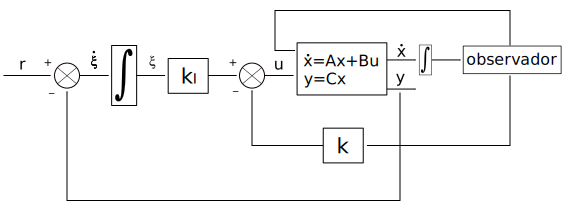
\includegraphics[scale=0.18]{Control de Sistemas Mecatronicos Figuras/15 Sin Integrador en la Planta.png}
        \caption{Sistema sin integrador en la planta}
\end{figure}

considere el sistema 
\[(1)
    \left\{
        \begin{array}{lll}
            \dot{x}(t) = Ax(t) + Bu(t) \\
            y(t) = Cx(t)
        \end{array}
    \right.
\]

Se define la entrada al sistema (1)
\[
    u = K_{I}\xi - kx
\]

Sustituye (2) en (1)
\[
    \begin{split}
        \dot{x} & = Ax + B(k_{I}\xi - kx) \\
        & = Ax + Bk_{I}\xi - Bkx \\
        & = (A-Bk)x + Bk_{I}\xi
    \end{split}
\]

Del integrador se puede ver que
\[
    \begin{split}
       \dot{\xi} & = r - y \\
       & = r - Cx \;\; (3) 
    \end{split}
\]

Usando (2) y (3) se puede formar el sistema en lazo cerrado
\[
    \begin{bmatrix}
        \dot{x} \\ \dot{\xi}
    \end{bmatrix} = 
    \begin{bmatrix}
        A-Bk & Bk_{I} \\
        -C & 0
    \end{bmatrix}
    \begin{bmatrix}
        x \\ \xi
    \end{bmatrix} + r
    \begin{bmatrix}
        0 \\ 1
    \end{bmatrix} \;\; (4)
\]

En estado estacionario la ecuación (4)
\[
    \begin{bmatrix}
        \lim_{t \to \infty}\dot{x}(t) \\
        \lim_{t \to \infty}\dot{\xi}(t)
    \end{bmatrix} = 
    \begin{bmatrix}
        A-Bk & Bk_{I} \\
        -C & 0
    \end{bmatrix}
    \begin{bmatrix}
        \lim_{t \to \infty}x(t) \\ 
        \lim_{t \to \infty}\xi(t)
    \end{bmatrix} + r
    \begin{bmatrix}
        0 \\ 1
    \end{bmatrix} \;\; (5)
\]

Haciendo (4) - (5)
\[
    \begin{bmatrix}
        \dot{x} - \lim_{t \to \infty}\dot{x}(t) \\
        \dot{\xi} - \lim_{t \to \infty}\dot{\xi}(t)
    \end{bmatrix} = 
    \begin{bmatrix}
        A-Bk & Bk_{I} \\
        -C & 0
    \end{bmatrix}
    \begin{bmatrix}
        x - \lim_{t \to \infty}x(t) \\ 
        \xi - \lim_{t \to \infty}\xi(t)
    \end{bmatrix} + r \;\; (6)
\]

Se define el error
\[
    \begin{split}
        e_{x} & = x - \lim_{t \to \infty} x(t) \\
        e_{\xi} & = \xi - \lim_{t \to \infty} \xi(t
    \end{split}
\]

Se reescribe el sistema (6)
\[
    \begin{bmatrix}
        \dot{e_{x}} \\
        \dot{e_{\xi}}
    \end{bmatrix} = 
    \begin{bmatrix}
        A-Bk & Bk_{I} \\
        -C & 0
    \end{bmatrix}
    \begin{bmatrix}
        e_{x} \\ 
        e_{\xi}
    \end{bmatrix}
\]

el sistema (6) se separa de la siguiente forma
\[
    \begin{split}
    \begin{bmatrix}
        \dot{e_{x}} \\
        \dot{e_{\xi}}
    \end{bmatrix} & = 
    \begin{bmatrix}
        A & 0 \\
        -C & 0
    \end{bmatrix}
    \begin{bmatrix}
        e_{x} \\ 
        e_{\xi}
    \end{bmatrix}
    + B
    \begin{bmatrix}
        -k & +k_{I}
    \end{bmatrix}
    \begin{bmatrix}
        e_{x} \\ 
        e_{\xi}
    \end{bmatrix} \\
    & =
    \begin{bmatrix}
        A & 0 \\
        -C & 0
    \end{bmatrix}
    \begin{bmatrix}
        e_{x} \\ 
        e_{\xi}
    \end{bmatrix}
    - B
    \underbrace{
        \begin{bmatrix}
            k & -k_{I}
        \end{bmatrix} 
                }_{\tilde{k}}
    \begin{bmatrix}
        e_{x} \\ 
        e_{\xi}
    \end{bmatrix}
    \end{split}
\]

donde 
\[ 
    e_{u} = -ke_{x} + k_{I}e_{\xi} = -\tilde{k} \begin{bmatrix}
        e_{x} \\ e_{\xi}
    \end{bmatrix} 
\]

También se puede ver de (1) en estado estacionario
\[
    \lim_{t \to \infty} u(t) = k_{I}\lim_{t \to \infty}\xi(t) - k\lim_{t \to \infty}x(t) (7)
\]

Haciendo (7) - (1)
\[
    \begin{split}
        u - \lim_{t \to \infty} u(t) & = k_{I}\xi - k_{I}\lim_{t \to \infty}\xi(t) - kx + k\lim_{t \to \infty}x(t) \\
        & = k_{I}(\xi - \lim_{t \to \infty}\xi(t)) - k(x - \lim_{t \to \infty}x(t)) \\
        & = K_{I}e_{\xi} - ke_{x}
    \end{split}
\]

Reescribiendo (4)
\[
    \begin{bmatrix}
        \dot{x} \\ \dot{\xi}
    \end{bmatrix} = 
    \begin{bmatrix}
        A & 0 \\
        -C & 0
    \end{bmatrix}
    \begin{bmatrix}
        x \\ \xi
    \end{bmatrix} +
    \begin{bmatrix}
        B \\ 0
    \end{bmatrix}u + r
    \begin{bmatrix}
        0 \\ 1
    \end{bmatrix} \;\; (8)  
\]

En estado estacionario (8)
\[
    \begin{bmatrix}
        \lim_{t \to \infty} \dot{x(t)} \\ 
        \lim_{t \to \infty} \dot{\xi} (t)
    \end{bmatrix} = 
    \begin{bmatrix}
        A & 0 \\
        -C & 0
    \end{bmatrix}
    \begin{bmatrix}
        \lim_{t \to \infty} x(t) \\
        \lim_{t \to \infty} \xi (t)
    \end{bmatrix} +
    \begin{bmatrix}
        B \\ 0
    \end{bmatrix} \lim_{t \to \infty} u(t) + r
    \begin{bmatrix}
        0 \\ 1
    \end{bmatrix} \;\; (9)
\]

Haciendo (8) - (9)
\[
    \begin{bmatrix}
        \dot{e_{x}} \\ 
        \dot{e_{\xi}}
    \end{bmatrix} = 
    \underbrace
    {
    \begin{bmatrix}
        A & 0 \\
        -C & 0
    \end{bmatrix}
    }_{\Tilde{A}}
    \begin{bmatrix}
        e_{x} \\
        e_{\xi}
    \end{bmatrix} +
    \underbrace{
        \begin{bmatrix}
            B \\ 0
        \end{bmatrix}
                }_{\tilde{B}}
    e_{u} \;\; (10)
\]

Se define la variable de estado como
\[
    E = 
    \begin{bmatrix}
        e_{x} \\ e_{\xi}
    \end{bmatrix}
\]

El sistema (10)
\[
    \dot{E} = \tilde{A}E + \tilde{B}e_{u} \;\; (11)
\]

Sustituyendo \( E \) en la definición de \( e_{u} \)
\[
    e_{u} = -\tilde{k}E \;\; (12)
\]

Sustituyendo (12) en (11)
\[
    \begin{split}
        \dot{E} & = \tilde{A}E + \tilde{B}(-\tilde{k}E) \\ 
        & = \tilde{A}E - \tilde{B}\tilde{k}E \\
        & = (\tilde{A} - \tilde{B}\tilde{k})E
    \end{split}
\]

Se resuelve como un problema de asignación de polos para la matriz \( \tilde{A} - \tilde{B}\tilde{k} \)